\subsection{Nesymetrické napájení}
\begin{figure}[h!]
    \centering
    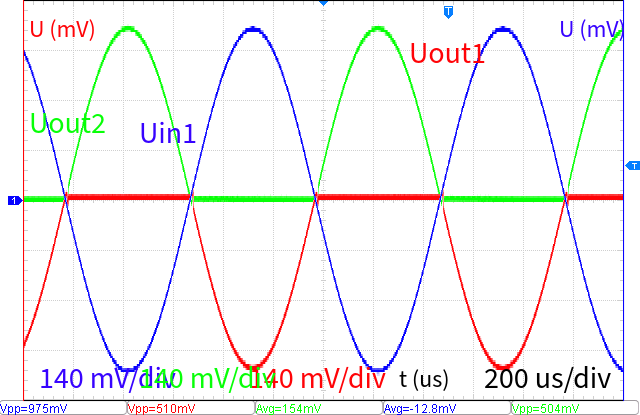
\includegraphics[width=0.8\textwidth]{lab/output1.png}
    \caption{Invertující zesilovač, nesym. napájení -- časový průběh správně zesíleného signálu.}
    \label{fig:lab/output1.png}
\end{figure}

\begin{figure}[h!]
    \centering
    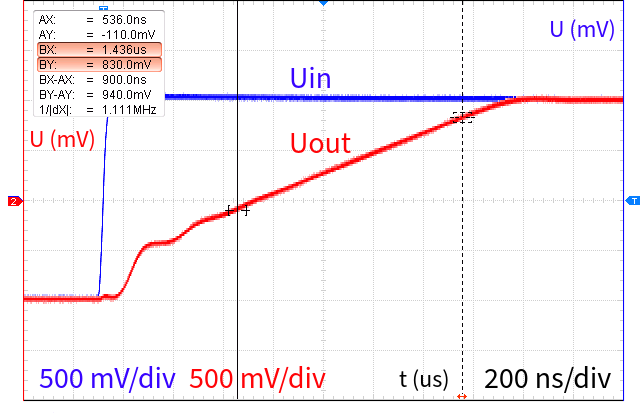
\includegraphics[width=0.8\textwidth]{lab/output2.png}
    \caption{Invertující zesilovač, nesym. napájení -- časový průběh správně zesíleného signálu, měřeno přímo na výstupu OZ, tedy s DC složkou.}
    \label{fig:lab-output2-png}
\end{figure}

\begin{figure}[h!]
    \centering
    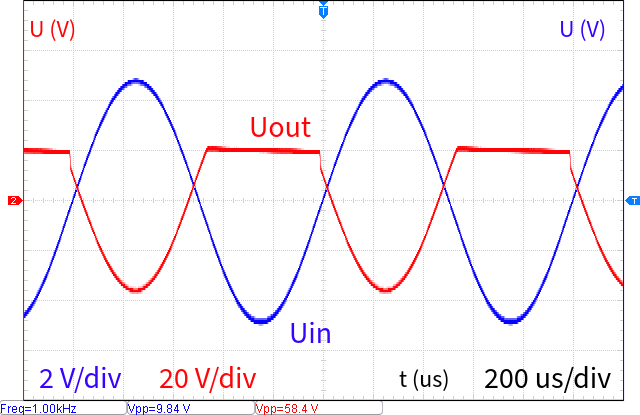
\includegraphics[width=0.8\textwidth]{lab/output3.png}
    \caption{Imvertující zesilovač, nesym. napájení -- vyšší amplituda vstupního signálu způsobila dosažení saturace.}
    \label{fig:lab-output3-png}
\end{figure}

\begin{figure}[h!]
    \centering
    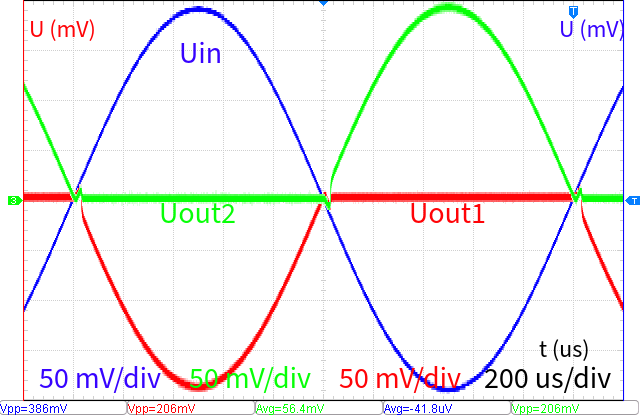
\includegraphics[width=0.8\textwidth]{lab/output4.png}
    \caption{lab/output4.png}
    \label{fig:lab-output4-png}
\end{figure}

\begin{figure}[h!]
    \centering
    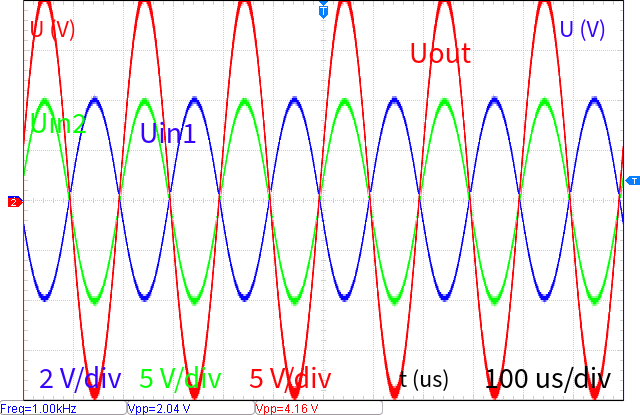
\includegraphics[width=0.8\textwidth]{lab/output5.png}
    \caption{lab/output5.png}
    \label{fig:lab-output5-png}
\end{figure}

\begin{figure}[h!]
    \centering
    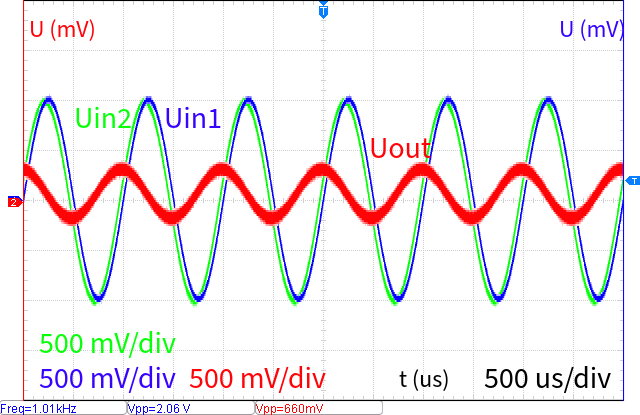
\includegraphics[width=0.8\textwidth]{lab/output6.png}
    \caption{lab/output6.png}
    \label{fig:lab-output6-png}
\end{figure}

\begin{figure}[h!]
    \centering
    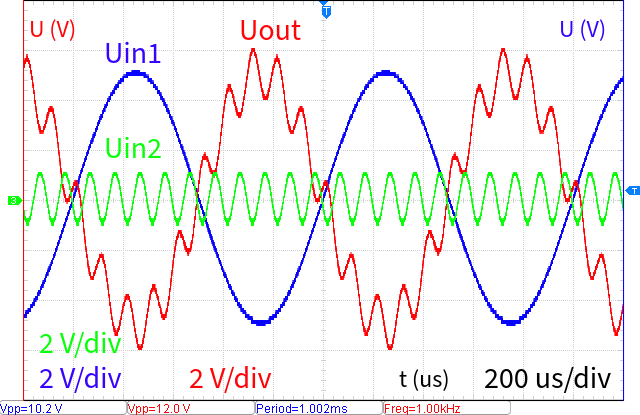
\includegraphics[width=0.8\textwidth]{lab/output7.png}
    \caption{lab/output7.png}
    \label{fig:lab-output7-png}
\end{figure}

\begin{figure}[h!]
    \centering
    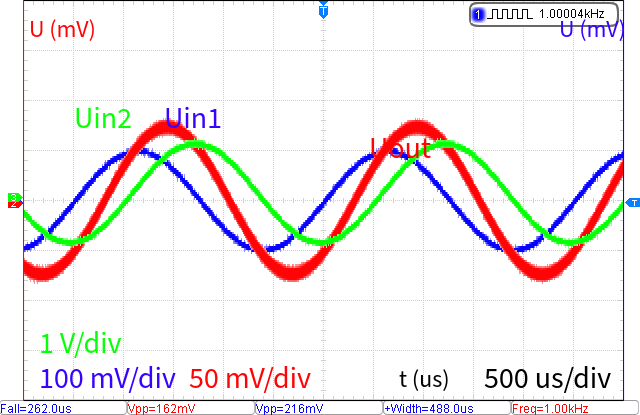
\includegraphics[width=0.8\textwidth]{lab/output8.png}
    \caption{lab/output8.png}
    \label{fig:lab-output8-png}
\end{figure}

\begin{figure}[h!]
    \centering
    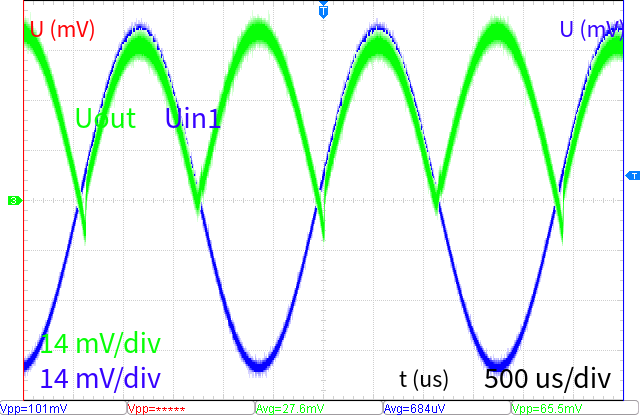
\includegraphics[width=0.8\textwidth]{lab/output9.png}
    \caption{lab/output9.png}
    \label{fig:lab-output9-png}
\end{figure}
